\RequirePackage{fix-cm}
%Journal of Mathematical Imaging and Vision
\documentclass[onecolumn]{svjour3}


\smartqed  % flush right qed marks, e.g. at end of proof

\usepackage{times}
\usepackage{bm,bbm}
\usepackage{amsmath,amssymb}
\usepackage{graphicx,subfigure}
\usepackage{url}
%\usepackage{units}
\usepackage{cite,balance}
\usepackage{comment}
\usepackage{multirow}
\usepackage{booktabs}
\usepackage{microtype}
\usepackage{siunitx}
\usepackage{color}
\usepackage{float}
%\usepackage{auto-pst-pdf}

\usepackage{mathptmx}

\usepackage{array}
\usepackage{varwidth}


\usepackage[normalem]{ulem} %%%% para tachar texto

%-----------------------
%Bibliography style
%\usepackage[numbers]{natbib}

%\newtheorem{definition}{Definition}
%\newtheorem{proposition}{Proposition}
\newcommand{\at}[2][]{#1|_{#2}}
%\newcommand{\K}{\text{K}}

\newcommand{\mc}[1]{\multicolumn{1}{c}{#1}}
\newcommand{\argmin}{\operatorname*{\text{arg min }}}

\begin{document}

\section{Nuevo gráfico corregido los IC}
\begin{figure}[hbt]
	\centering
	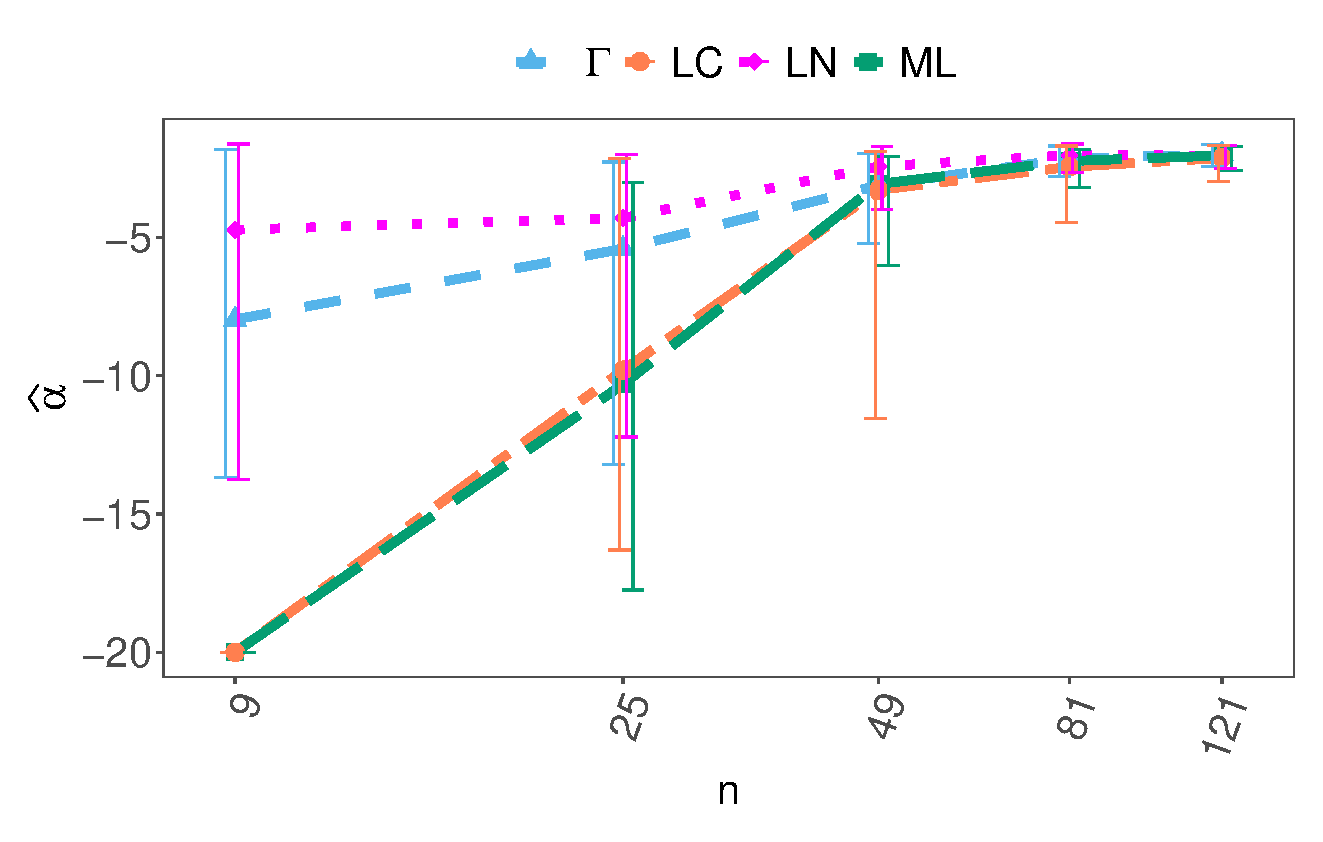
\includegraphics[width=0.7\linewidth]{../../../Figures/PaperTesis/AlfaVsTamCincoMuestrasCorregido_v2.eps}
	\caption{ $\widehat{\alpha}_{\text{{ML}}}$, $\widehat{\alpha}_{\Gamma}$, $\widehat{\alpha}_{\text{{LN}}}$ and $\widehat{\alpha}_{\text{{LC}}}$ for corresponding samples to image~\ref{CincoMuestras}.}\label{AlfaVsTamCincoMuestras}
\end{figure}

% Table generated by Excel2LaTeX from sheet 'IC'
\begin{table}[htbp]
	\centering
	\caption{\label{tab:LongIC}Length of confidence intervals showed in Fig.\ref{AlfaVsTamCincoMuestras}}
	\begin{tabular}{ccccc}
		\toprule 
		n     &  $\widehat{\alpha}_{\text{{ML}}}$    &  $\widehat{\alpha}_{\Gamma}$  &  $\widehat{\alpha}_{\text{{LN}}}$ &  $\widehat{\alpha}_{\text{{LC}}}$ \\
		\midrule
		9     &    -  & 11.86 & 12.12 & - \\
		25    & 14.74 & 10.94 & 10.20 & 14.14 \\
		49    & 3.94  & 3.25  & 2.28  & 9.65 \\
		81    & 1.38  & 1.09  & 1.03  & 2.75 \\
		121   & 0.85  & 0.77  & 0.83  & 1.31 \\
		 \bottomrule
	\end{tabular}
\end{table}%

\newpage

\section{Distribution of estimators, $\alpha=-3$ and $L=3$}
\begin{figure}[hbt]
	\centering
	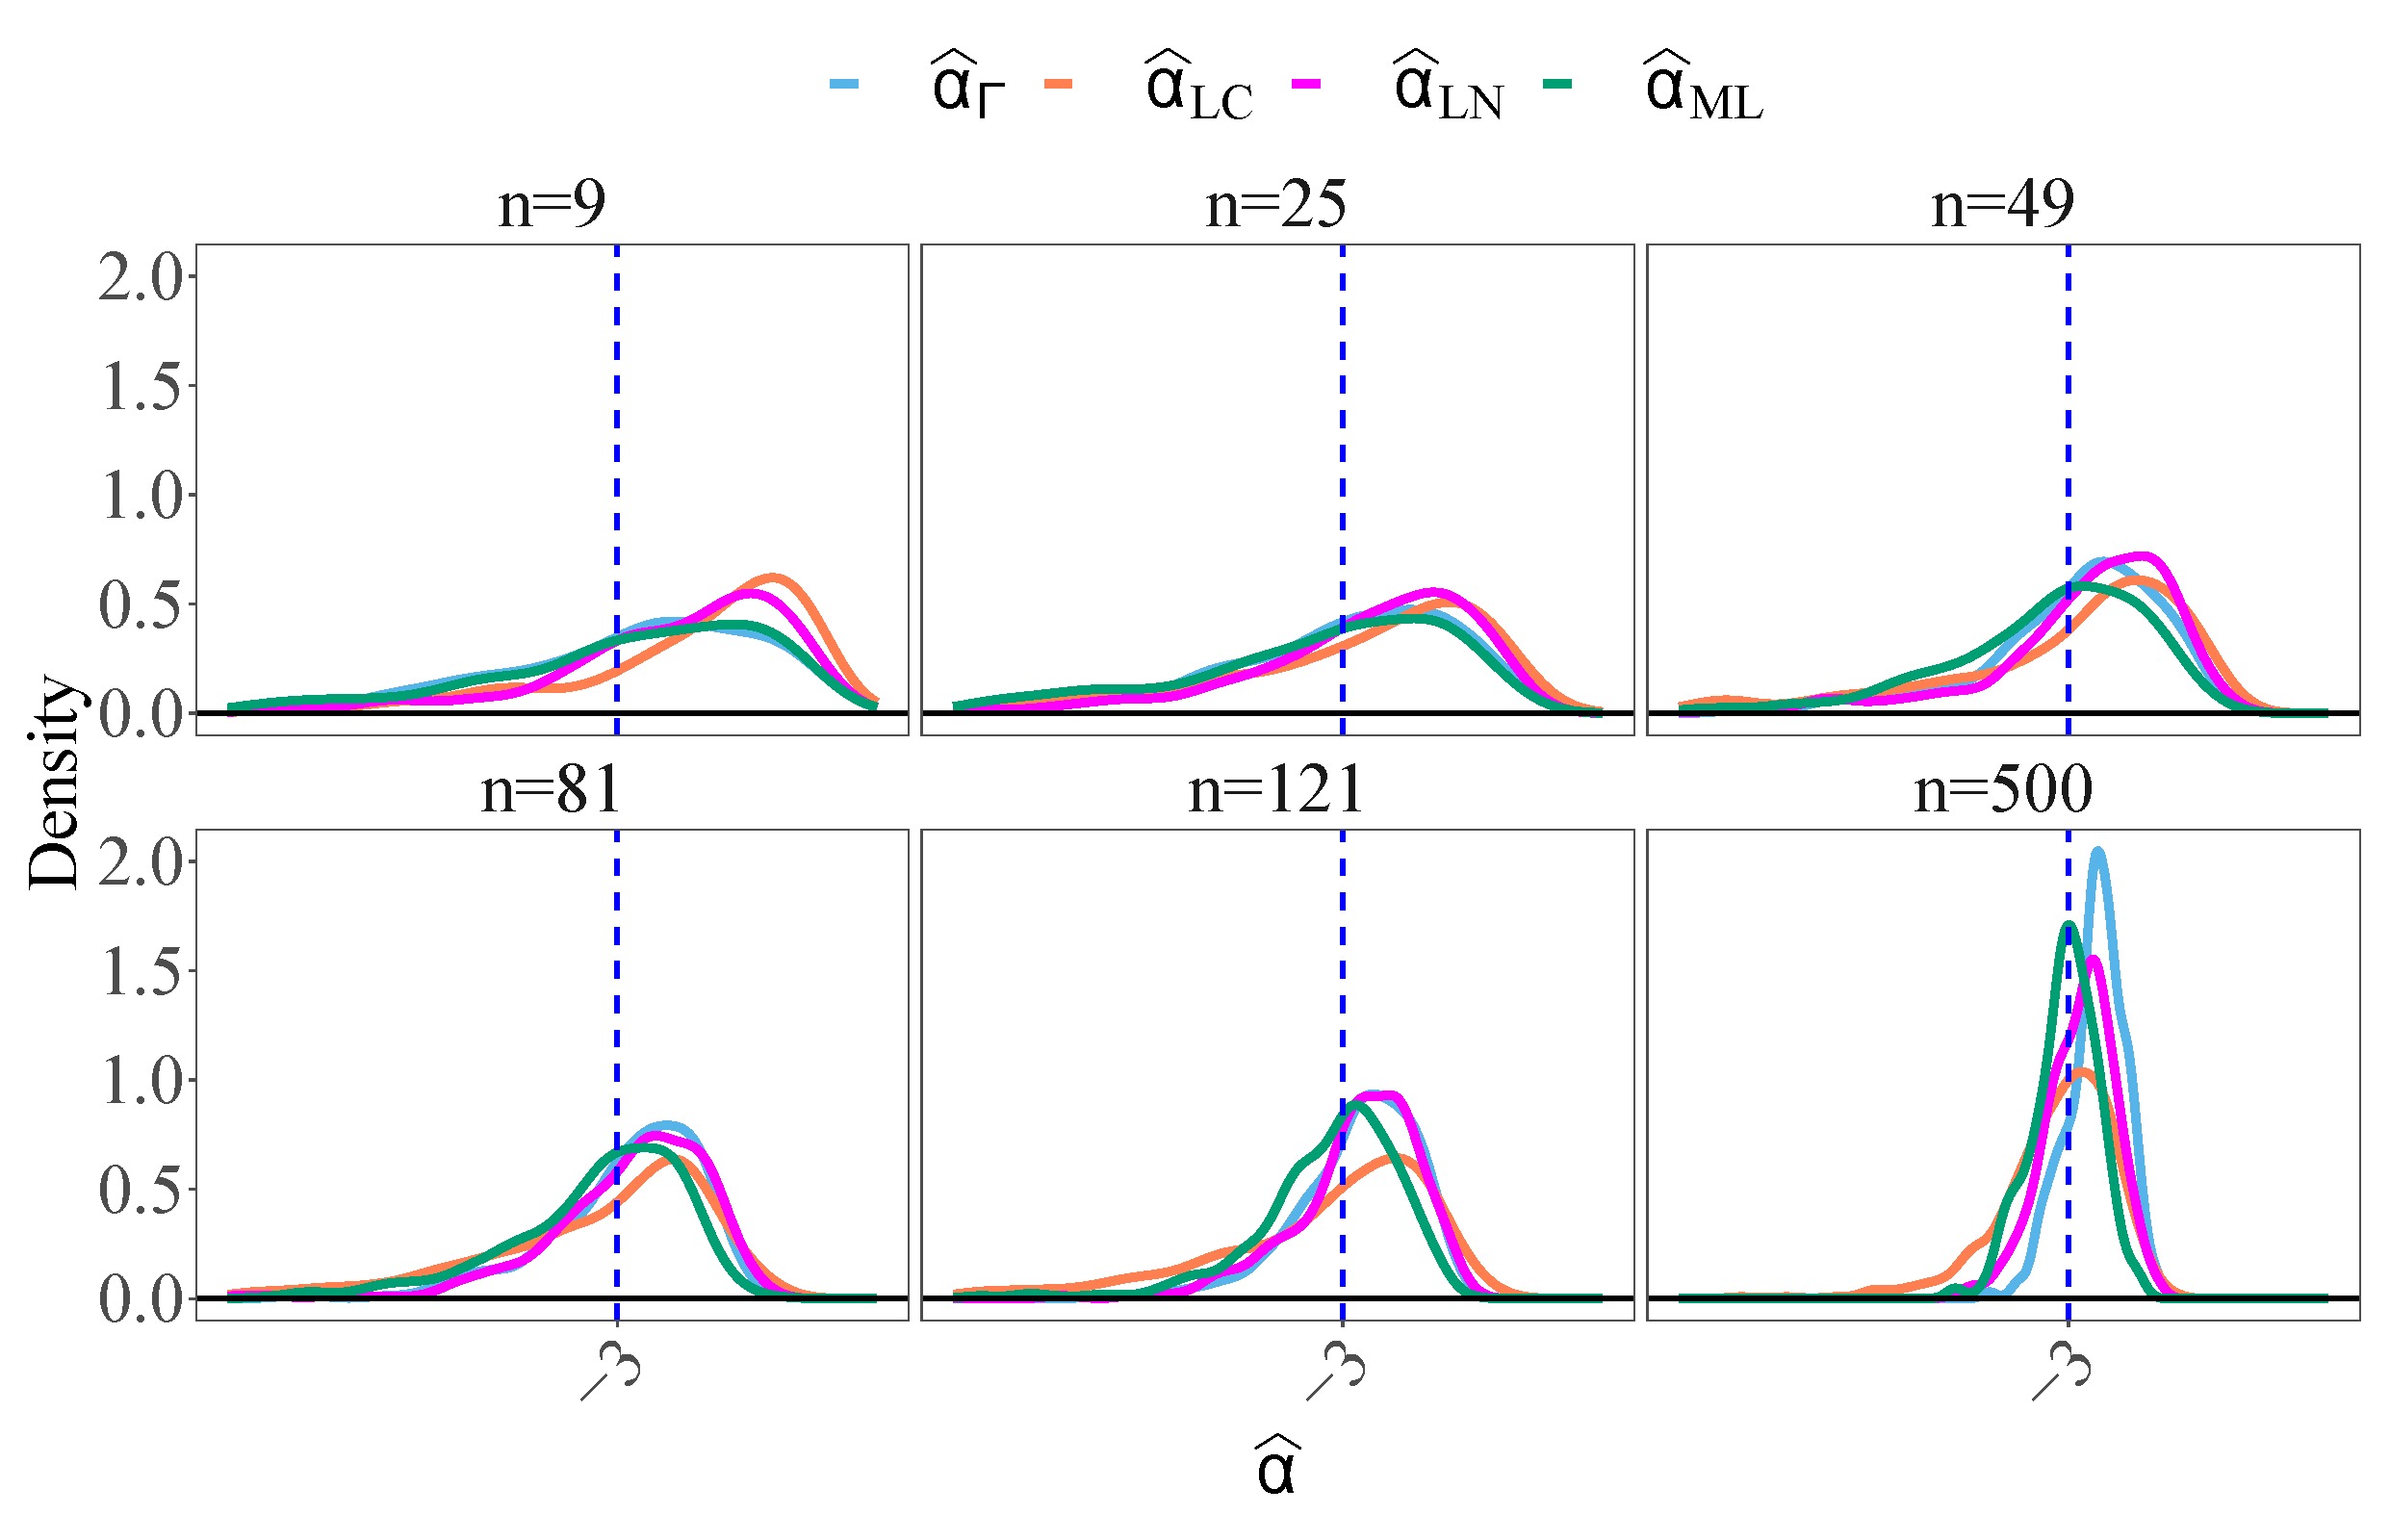
\includegraphics[width=0.7\linewidth]{../../../Figures/PaperTesis/DensidadEstimadorNoCont.eps}
	\caption{ Distribution of estimators, $\alpha=-3$ and  $L=3$ }\label{Fig:DistEstimator}
\end{figure}


\section{Skeweness, Kurtosis and Variance for simulated data, $L=3$}
\begin{table}[htbp]
	\centering
	\caption{Skeweness, Kurtosis and Variance for simulated data, $L=3$}
	\begin{tabular}{cc c*3{S[table-format=3.2]}  c*3{S[table-format=3.2]} c*3{S[table-format=3.2]}}
	\toprule
		\multirow{2}{5mm}{$\alpha$} & \multirow{2}{5mm}{$n$} & \multicolumn{4}{c}{Skewness}  & \multicolumn{4}{c}{Kurtosis}  & \multicolumn{4}{c}{Variance} \\
		\cmidrule(r){3-6} \cmidrule(r){7-10} \cmidrule(r){11-14}
			  &     & \multicolumn{1}{c}{$\widehat{\alpha}_{\text{{ML}}}$} & \multicolumn{1}{c}{$\widehat{\alpha}_{\Gamma}$} & \multicolumn{1}{c}{$\widehat{\alpha}_{\text{{LN}}}$}  & \multicolumn{1}{c}{$\widehat{\alpha}_{\text{{LC}}}$}  &  
			\multicolumn{1}{c}{$\widehat{\alpha}_{\text{{ML}}}$} & \multicolumn{1}{c}{$\widehat{\alpha}_{\Gamma}$} & \multicolumn{1}{c}{$\widehat{\alpha}_{\text{{LN}}}$}  & \multicolumn{1}{c}{$\widehat{\alpha}_{\text{{LC}}}$}  &
			\multicolumn{1}{c}{$\widehat{\alpha}_{\text{{ML}}}$} & \multicolumn{1}{c}{$\widehat{\alpha}_{\Gamma}$} & \multicolumn{1}{c}{$\widehat{\alpha}_{\text{{LN}}}$}  & \multicolumn{1}{c}{$\widehat{\alpha}_{\text{{C}}}$}  \\
%		$\alpha$  & $n$    &  $\widehat{\alpha}_{\text{{ML}}}$ & $\widehat{\alpha}_{\Gamma}$ & $\widehat{\alpha}_{\text{{LN}}}$ &  $\widehat{\alpha}_{\text{{LC}}}$  &  
%		$\widehat{\alpha}_{\text{{ML}}}$ & $\widehat{\alpha}_{\Gamma}$ & $\widehat{\alpha}_{\text{{LN}}}$ &  $\widehat{\alpha}_{\text{{LC}}}$  &  
%		$\widehat{\alpha}_{\text{{ML}}}$ & $\widehat{\alpha}_{\Gamma}$ & $\widehat{\alpha}_{\text{{LN}}}$ &  $\widehat{\alpha}_{\text{{LC}}}$\\
		\midrule
		\multirow{6}[2]{*}{-1.5} & 9     & -4.86 & -3.75 & -6.95 & -8.67 & 42.51 & 26.45 & 70.19 & 98.31 & 0.28  & 0.34  & 0.39  & 1.90 \\
		& 25    & -1.49 & -1.91 & -2.73 & -5.03 & 6.27  & 8.58  & 20.79 & 47.22 & 0.05  & 0.07  & 0.05  & 0.20 \\
		& 49    & -0.89 & -1.91 & -1.07 & -2.42 & 3.80  & 9.58  & 5.25  & 14.47 & 0.02  & 0.03  & 0.02  & 0.04 \\
		& 81    & -0.70 & -2.23 & -0.38 & -1.55 & 3.42  & 12.21 & 4.16  & 7.76  & 0.01  & 0.02  & 0.01  & 0.02 \\
		& 121   & -0.64 & -3.02 & 0.31  & -1.12 & 3.60  & 16.93 & 6.42  & 5.55  & 0.01  & 0.02  & 0.01  & 0.01 \\
		& 500   & -0.38 & -2.21 & 2.82  & -0.51 & 3.16  & 8.41  & 11.47 & 3.54  & 0.00  & 0.05  & 0.01  & 0.00 \\
		\midrule
		\multirow{6}[2]{*}{-3} & 9     & -2.39 & -2.36 & -3.42 & -3.38 & 10.28 & 11.25 & 17.03 & 15.95 & 5.58  & 2.21  & 5.30  & 8.03 \\
		& 25    & -3.07 & -4.64 & -4.12 & -2.99 & 15.68 & 37.20 & 26.88 & 13.94 & 5.03  & 2.46  & 2.40  & 5.90 \\
		& 49    & -3.87 & -4.54 & -4.34 & -3.70 & 30.93 & 43.69 & 31.26 & 22.17 & 1.62  & 0.85  & 1.31  & 3.93 \\
		& 81    & -1.52 & -1.84 & -1.86 & -3.09 & 6.52  & 9.81  & 9.28  & 15.13 & 0.54  & 0.39  & 0.44  & 3.28 \\
		& 121   & -2.33 & -1.36 & -2.17 & -4.09 & 15.12 & 6.88  & 15.10 & 33.19 & 0.36  & 0.23  & 0.27  & 1.67 \\
		& 500   & -0.46 & -0.53 & -0.53 & -1.29 & 3.29  & 3.31  & 3.33  & 6.21  & 0.06  & 0.05  & 0.07  & 0.19 \\
		\midrule
		\multirow{6}[2]{*}{-5} & 9     & -1.94 & -3.45 & -2.64 & -2.59 & 7.15  & 20.84 & 12.69 & 9.93  & 10.75 & 3.78  & 5.39  & 12.55 \\
		& 25    & -1.69 & -3.05 & -2.68 & -1.93 & 6.04  & 18.47 & 14.18 & 6.41  & 10.98 & 3.47  & 3.83  & 11.75 \\
		& 49    & -1.82 & -1.30 & -2.99 & -1.91 & 6.56  & 5.02  & 18.13 & 6.51  & 9.49  & 2.31  & 3.87  & 10.65 \\
		& 81    & -2.17 & -2.51 & -2.07 & -1.69 & 10.59 & 15.00 & 9.22  & 5.68  & 5.11  & 2.32  & 2.33  & 10.78 \\
		& 121   & -2.21 & -2.04 & -2.01 & -1.93 & 11.46 & 10.77 & 8.57  & 7.07  & 2.86  & 1.55  & 1.86  & 8.03 \\
		& 500   & -0.93 & -0.85 & -1.10 & -2.13 & 4.69  & 4.62  & 5.11  & 10.37 & 0.54  & 0.41  & 0.58  & 3.38 \\
		\midrule
		\multirow{6}[2]{*}{-8} & 9     & -1.55 & -2.68 & -2.69 & -2.20 & 4.83  & 14.01 & 11.81 & 8.00  & 16.17 & 3.65  & 6.92  & 11.56 \\
		& 25    & -0.96 & -2.50 & -2.11 & -1.67 & 3.29  & 13.58 & 8.68  & 5.12  & 13.94 & 4.50  & 6.28  & 15.44 \\
		& 49    & -1.12 & -2.17 & -1.92 & -1.50 & 3.63  & 9.71  & 7.90  & 4.65  & 15.18 & 5.05  & 5.75  & 13.45 \\
		& 81    & -1.09 & -1.82 & -1.69 & -1.35 & 3.52  & 8.34  & 7.35  & 4.21  & 13.25 & 5.32  & 5.09  & 15.29 \\
		& 121   & -1.17 & -1.35 & -1.71 & -1.26 & 4.15  & 5.38  & 7.07  & 4.27  & 10.02 & 4.50  & 5.25  & 12.02 \\
		& 500   & -1.33 & -1.26 & -1.52 & -1.35 & 6.21  & 6.11  & 7.39  & 4.50  & 3.27  & 1.95  & 2.72  & 10.24 \\
		\bottomrule
	\end{tabular}%
	\label{tab:addlabel}%
\end{table}%

\end{document}